\documentclass[10pt,a4paper]{article}
\usepackage[top=19mm,bottom=25.4mm,left=16mm,right=16mm]{geometry}
\usepackage{fontspec,graphicx,amsmath,amssymb,multicol,booktabs,array,tabularx}
\usepackage[hidelinks]{hyperref}
\setmainfont{Times New Roman}
\setlength{\columnsep}{6mm}
\setlength{\parindent}{0pt}
\setlength{\parskip}{3pt}
\setlength{\multicolsep}{4pt}
\setlength{\abovedisplayskip}{4pt}
\setlength{\belowdisplayskip}{4pt}
\pagestyle{empty}
\makeatletter
\renewcommand{\section}{\@startsection{section}{1}{0pt}{5pt}{2pt}{\normalfont\normalsize\bfseries}}
\makeatother
\newcommand{\sect}[1]{\section*{#1}}
\begin{document}
\begin{center}
\includegraphics[width=\textwidth]{baic2026_header.png}\par\vspace{4pt}
{\fontsize{14}{17}\selectfont\bfseries Hard-Budget Feature Selection with Resampled Mutual-Information Repair in EHOA}\par
Amirreza Ghaffarian\par
Graduate Student, Islamic Azad University\end{center}
\textbf{Abstract. } We compare four budget repairs within the Enhanced Hiking Optimization Algorithm (EHOA) while preserving its search and wrapper objective. The proposed repair ranks features by a nonnegative mean-minus-standard-deviation mutual-information score divided by synthetic acquisition cost. This score is a conservative heuristic, not a calibrated confidence bound. We audit 300 archived runs on ten classification datasets. All 240 constrained outputs satisfy a budget of 30\% of total feature cost. Source inspection identifies target leakage in Steel Plates and a subject-overlap risk in Parkinsons; we exclude both from the main retrospective analysis. Across eight eligible datasets, resampled repair changes mean balanced accuracy from 0.8068 to 0.8116, cost ratio from 0.4791 to 0.2792, and Nogueira stability from 0.1161 to 0.2550. Friedman tests detect method differences in cost and stability, but not balanced accuracy. The resampled-versus-EHOA stability contrast does not survive within-metric Holm correction. A breast-cancer cytology case illustrates subset selection without claiming clinical validation or monetary savings. The contribution is an auditable repair comparison, not general predictive superiority. A separate 60-run exploratory correction also finds no general predictive advantage.

\textbf{Keywords. } feature selection, hard budget, resampled mutual information, subset stability
\begin{multicols}{2}\raggedcolumns
\sect{1  Problem and contribution}
A small feature set need not be inexpensive: acquisition costs can differ between variables. Hard-budget selection limits the sum of selected costs [1]. Subset stability measures how feature choices vary across training samples and random search, rather than how accuracy or convergence varies [2]. In biomedical classification, this distinction matters when investigators interpret a selected measurement panel.

Medical feature selection spans imaging, signals and molecular data [3]. Predictive discrimination, reproducible feature identity and acquisition burden are separate objectives. Correlated descriptors can substitute for one another, so a changing mask need not imply poor prediction; conversely, a repeated mask does not establish a valid biomarker. This motivates reporting balanced accuracy, cost and chance-corrected subset stability together.

We retain the implemented EHOA search [4] and compare unconstrained EHOA with four repairs. Only the repair utility changes among constrained variants. The contribution is the integration and controlled evaluation of resampled relevance-per-cost repair. We do not claim that budgets, repair, mutual information (MI), or resampling are new. CostStableEHOA remains the code identifier; the revised title avoids implying stable costs or proven selection stability.

\sect{2  Related studies}
Stability metrics can reward reproducible yet weak predictors; importance-weighted stability addresses this concern [5]. Medical budget selection with penalized risk [6], sequential acquisition [7], and grouped costs with shadow features [8] solve related but different problems. Table 1 summarizes these distinctions; NR means not reported in the inspected source. Their numerical results are not directly comparable with our protocol.

\par\vspace{3pt}\begin{minipage}{\linewidth}{\footnotesize Table 1. Related-work comparison. Full evaluation details are in the supplement.\par}
{\fontsize{6.8}{8.3}\selectfont\setlength{\tabcolsep}{2pt}\renewcommand{\arraystretch}{1.1}
\begin{tabularx}{\linewidth}{>{\hsize=1.0000\hsize\raggedright\arraybackslash}X>{\hsize=1.0000\hsize\raggedright\arraybackslash}X>{\hsize=1.0000\hsize\raggedright\arraybackslash}X>{\hsize=1.0000\hsize\raggedright\arraybackslash}X>{\hsize=1.0000\hsize\raggedright\arraybackslash}X>{\hsize=1.0000\hsize\raggedright\arraybackslash}X}\toprule
Study & Budget & Costs & Stability & Evaluation & Difference\\\midrule
Jagdhuber [1] & Yes & Additive & NR & Simulation & Feasible GA\\
Nogueira [2] & NR & NR & Chance-corrected & Resampling & Metric\\
Hamer [5] & NR & NR & Importance-weighted & Resampling & Metric limits\\
Klonecki [6] & Yes & Feature / proxy & NR & Medical data & Penalized ERM\\
Valancius [7] & NR & Sequential & NR & AFA benchmarks & Patient-wise policy\\
Klonecki [8] & Yes & Grouped & NR & MIMIC & Shadow stopping\\
This work & Yes & Synthetic additive & Nogueira & 2 x 3 outer & MI/cost repair\\
\bottomrule\end{tabularx}}
\end{minipage}\par\vspace{3pt}
Classical stability selection aggregates repeated subsample selections and, under specified assumptions and thresholds, controls false selections [9,10]. Our four MI resamples instead estimate a deletion utility before wrapper search. We neither threshold repeated selection probabilities nor inherit those error-control guarantees. Nogueira stability evaluates the final masks [2]; it is not the optimized fitness. Active acquisition [7] chooses measurements sequentially per case, whereas our repair returns a fixed feasible subset.

\sect{3  Implemented EHOA}
Each hiker has a continuous position x and a velocity v; a binary mask z selects features. Initialization uses a tent sequence with initial value 0.7 and parameter 0.4, mapped to [-6,6]. Velocities start uniformly in [-1.2,1.2]. For iteration t of T=10, the implemented update is:

\begin{equation}\begin{gathered}\begin{aligned}v_i\leftarrow\operatorname{clip}_{[-12,12]}\big(&w_t v_i+SF_t[2r_1(p_i-x_i)\\&+2r_2(g-x_i)]\big)\end{aligned}\end{gathered}\end{equation}
\begin{equation}\begin{gathered}\begin{gathered}x_i\leftarrow\operatorname{clip}_{[-6,6]}(x_i+v_i)\\w_t=0.9-0.5t/T,\quad SF_t=3-2t/T\end{gathered}\end{gathered}\end{equation}
Here p\_i and g are personal and global best continuous positions, and r\_1,r\_2 are independent per-feature uniform draws. The sigmoid gives selection probability 1/(1+exp(-x\_j)); an empty sampled mask restores the largest probability. The implementation keeps continuous leaders separate from repaired masks, caches fitness for duplicate masks, and stops after ten iterations without early stopping.

\sect{4  Budget repair and stability}
Costs are fixed positive additive synthetic units, independent of labels: c is drawn once per dataset from lognormal(0,0.7), with NumPy seed 1000+D. The absolute budget B=0.30 sum(c) is derived from a relative budget. Ionosphere and Dermatology share a cost vector because both have D=34. A nonempty mask is feasible when sum(z\_j c\_j) <= B.

\begin{equation}\begin{gathered}u_j=\max(0,\bar I_j-\lambda s_j),\qquad q_j=u_j/c_j,\qquad\lambda=1\end{gathered}\end{equation}
For resampled repair, four within-class samples draw ceil(0.8 n\_class) rows with replacement (minimum two). Dense mutual\_info\_classif uses continuous-feature estimation, three neighbors, and nats; missing values are zero-filled for MI only. s\_j is the sample standard deviation (ddof=1). No division by sqrt(R) or calibrated confidence level occurs. Utility is computed once on the outer-training partition using a separate RNG seeded by selector\_seed+7919.

\par\vspace{3pt}\begin{minipage}{\linewidth}{\footnotesize Table 2. Four repairs share the same deletion rule.\par}
{\fontsize{6.8}{8.3}\selectfont\setlength{\tabcolsep}{2pt}\renewcommand{\arraystretch}{1.1}
\begin{tabularx}{\linewidth}{>{\hsize=1.0000\hsize\raggedright\arraybackslash}X>{\hsize=1.0000\hsize\raggedright\arraybackslash}X>{\hsize=1.0000\hsize\raggedright\arraybackslash}X}\toprule
Repair & Utility u\_j & Meaning\\\midrule
Random/cost & U(0,1), fixed per fit & Not uniform deletion\\
Cheapest & 1 & Largest cost first\\
MI/cost & Single-sample MI & Relevance per cost\\
Resampled/cost & max(0, mean MI - SD) & Conservative heuristic\\
\bottomrule\end{tabularx}}
\end{minipage}\par\vspace{3pt}
Procedure: initialize population; sample sigmoid mask; repair before fitness; evaluate; update personal/global leaders; repeat movement, sampling, repair, and evaluation; return the best repaired mask. Repair removes argmin(q\_j) among active features while cost exceeds B and more than one feature remains. An unaffordable singleton is cleared; an empty mask restores the affordable feature maximizing q\_j. A tie selects the first feature index. Utility is never recomputed per candidate.

\begin{equation}\begin{gathered}F(z)=0.99(1-\overline{Acc}_{inner})+0.01\|z\|_0/D\end{gathered}\end{equation}
The unchanged objective minimizes ordinary inner accuracy error, not balanced-accuracy error. External balanced accuracy (BA) is the mean recall across classes. Stability is computed once per dataset/method from M=6 final masks:

\begin{equation}\begin{gathered}\Phi=\operatorname{clip}_{[-1,1]}\left(1-\frac{\frac{M}{M-1}\frac{1}{D}\sum_j p_j(1-p_j)}{(\bar k/D)(1-\bar k/D)}\right)\end{gathered}\end{equation}
p\_j is selection frequency and k-bar is mean subset size. Identical empty/full masks return one in the code. This dimensionless chance-corrected outcome [2] mixes data-split and search variation; overlapping training folds make the six masks dependent. We do not treat copied stability values in six CSV rows as six observations. Jaccard overlap is supplementary and is not chance-corrected.

The continuous-discrete nearest-neighbor MI estimator [11] measures marginal dependence, not conditional contribution after other features are selected. Univariate ranking can retain redundant correlated variables or discard features useful only jointly. With four resamples, the estimated spread is imprecise; lambda=1 expresses a fixed penalty rather than a coverage probability. These design limits motivate comparison with the simpler single-MI and cheapest repairs, rather than attributing every difference to stability.

Feasibility follows from positive costs and finite deletion: every deletion reduces both subset size and total cost. An unaffordable last feature is cleared; restoration chooses only an individually affordable feature. Thus a nonempty feasible output exists when at least one feature costs at most B, as verified for these datasets. This proves budget compliance, not optimal utility or accuracy. Repair may remove a jointly useful feature because its ranking is marginal and fixed. Repeated repair also maps different search positions to the same mask; cached fitness avoids evaluating such duplicates again.

\sect{5  Datasets and source audit}
\par\vspace{3pt}\begin{minipage}{\linewidth}{\footnotesize Table 3. Snapshot / deduplicated N; D is the supplied numeric feature count.\par}
{\fontsize{6.8}{8.3}\selectfont\setlength{\tabcolsep}{2pt}\renewcommand{\arraystretch}{1.1}
\begin{tabularx}{\linewidth}{>{\hsize=1.4237\hsize\raggedright\arraybackslash}X>{\hsize=1.3220\hsize\raggedright\arraybackslash}X>{\hsize=0.3559\hsize\raggedright\arraybackslash}X>{\hsize=0.3051\hsize\raggedright\arraybackslash}X>{\hsize=1.9322\hsize\raggedright\arraybackslash}X>{\hsize=0.6610\hsize\raggedright\arraybackslash}X}\toprule
Dataset & N raw/used & D & K & Class counts used & Source\\\midrule
Breast Cancer & 569 / 569 & 30 & 2 & 212/ 357 & U17\\
Wine & 178 / 178 & 13 & 3 & 59/ 71/ 48 & U109\\
Ionosphere & 351 / 350 & 34 & 2 & 125/ 225 & O59\\
Sonar & 208 / 208 & 60 & 2 & 111/ 97 & O40\\
Dermatology & 366 / 366 & 34 & 6 & 112/ 61/ 72/ 49/ 52/ 20 & O35\\
Spambase & 4601 / 4210 & 57 & 2 & 2531/ 1679 & O44\\
Parkinsons* & 195 / 195 & 22 & 2 & 48/ 147 & O1488\\
Hill-Valley & 1212 / 1212 & 100 & 2 & 606/ 606 & O1479\\
Steel Plates* & 1941 / 1941 & 33 & 2 & 1268/ 673 & O1504\\
Madelon & 2600 / 2600 & 500 & 2 & 1300/ 1300 & O1485\\
\bottomrule\end{tabularx}}
\end{minipage}\par\vspace{3pt}
U identifiers link to archive.ics.uci.edu/dataset/\{id\}; O identifiers link to openml.org/d/\{id\}. The supplement gives clickable direct links, raw/used class counts, hashes and budgets. No runtime one-hot encoding occurs. Steel has 33 inputs and two classes in the snapshot, whereas UCI defines 27 predictors and seven fault types. Its V28-V33 are six fault indicators and exactly determine the target; we exclude these results. Parkinsons is a recording-level dataset with repeated participants and no subject-group split; we also exclude it from the main analysis. Eight eligible datasets retain 240 runs.

\sect{6  Evaluation and statistical analysis}
SMOTE creates synthetic minority-class training examples [12]; it does not increase the number of independent test subjects. Model selection must remain separate from performance estimation [13]. Here the inner score guides search, while untouched outer tests provide the reported predictions. MI sees the full outer-training labels, including inner-validation labels; thus the inner score is not an unbiased validation estimate. The corrected subject splits address recording overlap, but do not change this utility design.

Table 4 documents actual settings rather than class defaults. All methods share data splits, costs, seeds, search equations and wrapper fitness. Initialization positions are deterministic; search velocities and masks use the selector RNG. The four repairs therefore isolate utility ranking under a common budget; unconstrained EHOA additionally tests the effect of imposing that budget.

\par\vspace{3pt}\begin{minipage}{\linewidth}{\footnotesize Table 4. Settings extracted from code and configuration.\par}
{\fontsize{6.8}{8.3}\selectfont\setlength{\tabcolsep}{2pt}\renewcommand{\arraystretch}{1.1}
\begin{tabularx}{\linewidth}{>{\hsize=1.0000\hsize\raggedright\arraybackslash}X>{\hsize=1.0000\hsize\raggedright\arraybackslash}X}\toprule
Parameter & Value\\\midrule
Population / iterations & 8 / 10; no early stop\\
Position / velocity clip & [-6,6] / [-12,12]\\
Tent / sweep / inertia & 0.7, p=0.4 / 3 to 1 / 0.9 to 0.4\\
c1,c2 / alpha & 2,2 / 0.99\\
Outer / inner folds & 3 stratified / 3 stratified\\
Outer seeds & 71001, 71002\\
Selector seed & outer seed + fold index x 100003\\
MI resamples / fraction & 4 / 0.8 with replacement\\
lambda / MI neighbors & 1 / 3\\
Cost / budget & lognormal(0,0.7) / 30\% total\\
Classifier & 5-NN; uniform; Euclidean\\
Imputation / scale & Training mean / StandardScaler\\
SMOTE & Training only; k=min(5,n\_min-1)\\
\bottomrule\end{tabularx}}
\end{minipage}\par\vspace{3pt}
Within each inner fold, training data alone fit mean imputation, scaling and SMOTE; validation rows remain unchanged. MI utility uses all outer-training labels, including rows that later become inner validation. Thus inner scores are selection scores, not unbiased estimates. Outer-test labels do not enter selection. Final outer training fits preprocessing/SMOTE and 5-NN; archived metrics retain only 5-NN although the runner fits four classifiers. Preprocessing and SMOTE occur before masking; this is a simulation, not a deployed selected-only acquisition pipeline.

We average six BA/cost/size values per dataset and use one stability value per method/dataset. Eight datasets, not 240 rows, are analysis blocks [14]. The 2026-10-12 analysis is retrospective: the supplied confirmatory flag and config hash do not establish dated preregistration. We use tie-corrected Friedman tests (df=4), two-sided paired Wilcoxon contrasts of resampled repair versus four controls, and Holm correction within each metric. The supplement also corrects all 24 contrasts and six omnibus tests. Dataset-bootstrap intervals (20,000 draws; seed 20261012) are descriptive, unadjusted percentile intervals.

\sect{7  Results}
\par\vspace{3pt}\begin{minipage}{\linewidth}{\footnotesize Table 5. Equal-weight means over eight eligible datasets; V is final budget exceedance.\par}
{\fontsize{6.8}{8.3}\selectfont\setlength{\tabcolsep}{2pt}\renewcommand{\arraystretch}{1.1}
\begin{tabularx}{\linewidth}{>{\hsize=1.0000\hsize\raggedright\arraybackslash}X>{\hsize=1.0000\hsize\raggedright\arraybackslash}X>{\hsize=1.0000\hsize\raggedright\arraybackslash}X>{\hsize=1.0000\hsize\raggedright\arraybackslash}X>{\hsize=1.0000\hsize\raggedright\arraybackslash}X>{\hsize=1.0000\hsize\raggedright\arraybackslash}X}\toprule
Method & BA & Cost ratio & Size & Stability & V\\\midrule
EHOA & 0.8068 & 0.4791 & 49.21 & 0.1161 & 47/48\\
Random/cost & 0.8054 & 0.2727 & 37.54 & 0.1238 & 0/48\\
Cheapest & 0.8090 & 0.2708 & 41.50 & 0.2423 & 0/48\\
MI/cost & 0.8109 & 0.2770 & 32.65 & 0.2287 & 0/48\\
Resamp./cost & 0.8116 & 0.2792 & 36.40 & 0.2550 & 0/48\\
\bottomrule\end{tabularx}}
\end{minipage}\par\vspace{3pt}
\par\vspace{3pt}\begin{minipage}{\linewidth}{\footnotesize Table 6. Friedman statistic and raw p; average ranks in E/R/C/M/S order, 1 is best.\par}
{\fontsize{6.8}{8.3}\selectfont\setlength{\tabcolsep}{2pt}\renewcommand{\arraystretch}{1.1}
\begin{tabularx}{\linewidth}{>{\hsize=1.0000\hsize\raggedright\arraybackslash}X>{\hsize=1.0000\hsize\raggedright\arraybackslash}X>{\hsize=1.0000\hsize\raggedright\arraybackslash}X>{\hsize=1.0000\hsize\raggedright\arraybackslash}X>{\hsize=1.0000\hsize\raggedright\arraybackslash}X>{\hsize=1.0000\hsize\raggedright\arraybackslash}X>{\hsize=1.0000\hsize\raggedright\arraybackslash}X>{\hsize=1.0000\hsize\raggedright\arraybackslash}X}\toprule
Metric & Chi2 & p & E & R & C & M & S\\\midrule
BA & 4.5000 & 0.34255 & 3.12 & 3.88 & 3.00 & 2.75 & 2.25\\
Cost & 21.1000 & 0.00030 & 5.00 & 1.88 & 1.88 & 3.00 & 3.25\\
Size & 23.7233 & 0.00009 & 5.00 & 1.88 & 3.81 & 2.06 & 2.25\\
Stability & 15.7000 & 0.00345 & 4.25 & 4.12 & 1.88 & 2.50 & 2.25\\
\bottomrule\end{tabularx}}
\end{minipage}\par\vspace{3pt}
Resampled repair versus EHOA changes cost ratio by -0.19986 (Wilcoxon W=0, raw p=0.00781; within-metric Holm p=0.03125; rank-biserial r=-1). Stability changes by +0.13895 (W=1, raw p=0.01563; Holm p=0.06250; r=0.944). BA changes by +0.00482 (W=9; Holm p=0.750; r=0.500; 95\% interval [-0.00149,0.01109]). Neither equivalence nor non-inferiority follows. No resampled repair contrast with the other three repairs is significant within metric for BA or Nogueira stability.

As a separate exploratory sensitivity analysis, we completed 60 corrected runs: Steel used 27 predictors and seven classes; Parkinsons used subject-disjoint outer and inner folds after matching all 195 recordings to the UCI file. Combining these with the 240 eligible archived runs gives ten corrected dataset blocks. Friedman BA remains nonsignificant (Chi2=4.32, df=4, p=0.36443). Resampled-versus-EHOA stability has within-metric Holm p=0.01563, but Holm over all 20 contrasts gives p=0.06641. Mean BA delta is -0.00583, with descriptive interval [-0.02523,0.00771]. These new exploratory results neither validate the original leaked experiment nor establish superiority over simpler repairs.

\par\begin{minipage}{\linewidth}\centering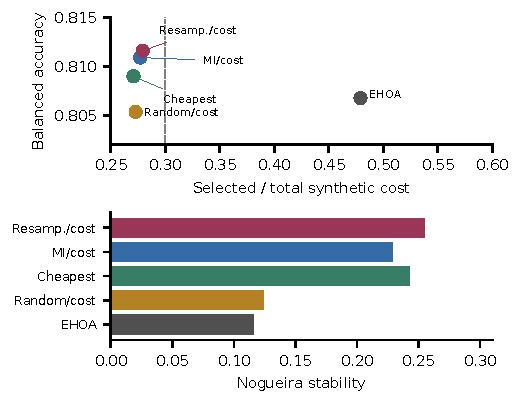
\includegraphics[width=\linewidth]{figures/eligible_comparison.pdf}\par{\footnotesize Figure 1. Eight-dataset means; cost uses synthetic units. Stability bars do not imply significant pairwise differences.\par}\end{minipage}\par
\sect{8  Biomedical case and congress relevance}
The UCI diagnostic breast-cancer dataset contains 569 fine-needle-aspirate cases (212 malignant, 357 benign) and 30 nuclear-image descriptors [15]. Radius, texture, perimeter, area, smoothness, compactness, concavity, concave points, symmetry and fractal dimension each have mean, error and worst summaries. Table 7 illustrates the five methods on this dataset.

\par\vspace{3pt}\begin{minipage}{\linewidth}{\footnotesize Table 7. Breast-cancer case, means over six runs.\par}
{\fontsize{6.8}{8.3}\selectfont\setlength{\tabcolsep}{2pt}\renewcommand{\arraystretch}{1.1}
\begin{tabularx}{\linewidth}{>{\hsize=1.0000\hsize\raggedright\arraybackslash}X>{\hsize=1.0000\hsize\raggedright\arraybackslash}X>{\hsize=1.0000\hsize\raggedright\arraybackslash}X>{\hsize=1.0000\hsize\raggedright\arraybackslash}X>{\hsize=1.0000\hsize\raggedright\arraybackslash}X}\toprule
Method & BA & Cost ratio & Size & Stability\\\midrule
EHOA & 0.9563 & 0.5227 & 14.17 & 0.0682\\
Random/cost & 0.9452 & 0.2651 & 10.17 & 0.0627\\
Cheapest & 0.9557 & 0.2673 & 11.33 & 0.2815\\
MI/cost & 0.9462 & 0.2758 & 10.50 & 0.2137\\
Resamp./cost & 0.9525 & 0.2799 & 11.17 & 0.2059\\
\bottomrule\end{tabularx}}
\end{minipage}\par\vspace{3pt}
\par\begin{minipage}{\linewidth}\centering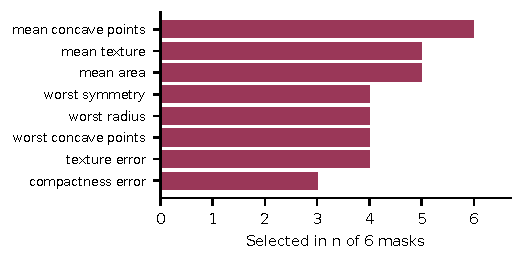
\includegraphics[width=\linewidth]{figures/breast_top_frequencies.pdf}\par{\footnotesize Figure 2. Selection counts for the eight most frequent resampled-repair features, from six archived masks.\par}\end{minipage}\par
Resampled repair selects mean concave points in 6/6 masks and mean texture and mean area in 5/6. These counts describe the archived selections; they do not establish causal biomarkers or clinical reliability. Cheapest repair has greater stability here (0.2815 versus 0.2059). Synthetic feature costs are not biopsy prices; all descriptors derive from the same acquisition, so grouped measurement costs would be more realistic.

The closest official BAIC2026 topic is Artificial Intelligence, Machine Learning and Data Science / Intelligent Disease Diagnosis Systems (baic.um.ac.ir/fa/home/Content/12). Our biomedical contribution concerns computational measurement-panel selection, not a clinically validated diagnostic system. We claim no cognitive-science mechanism.

Across the eight datasets, the proposed repair reduces mean synthetic cost by 41.7\% and subset size by 26.0\% relative to unconstrained EHOA. These comparisons include imposing a budget on an otherwise infeasible baseline: 47 of its 48 outputs exceed that budget. They cannot isolate a benefit of resampling. The cheapest repair already attains mean cost 0.2708 and stability 0.2423, compared with 0.2792 and 0.2550 for resampled repair. The small descriptive stability difference is not corrected pairwise evidence. A medical panel decision therefore needs measured acquisition groups and acceptable sensitivity, rather than choosing the method from stability alone.

\sect{9  Limitations and reproducibility}
Only one synthetic budget, four MI resamples, eight eligible datasets, two seeds and a short search were assessed. Ordinal Dermatology inputs are treated as continuous by MI; duplicated bootstrap rows can distort nearest-neighbor MI. Overlap-based stability does not verify clinical importance. The corrected exploratory follow-up is reported separately. UCI describes 31 Parkinson participants, but its file contains 32 distinct subject prefixes; group identity needs independent confirmation. Dated registration, original execution logs and end-to-end timing are unavailable; runtime\_seconds excludes MI utility construction in constrained methods.

The accompanying local supplement contains all dataset links, 300 mask audits, per-dataset outcomes, cost vectors, statistics and regeneration scripts. Raw files and originals remain intact. No verified public code repository is supplied, and local availability is not public release. The eight-dataset exclusion and analysis are retrospective, not new confirmatory experiments.

\sect{10  Conclusion}
All archived constrained outputs are budget-feasible. On eight eligible datasets, resampled repair shows a descriptive cost-stability trade-off but no corrected pairwise stability advantage or general predictive superiority. A stronger biomedical claim requires grouped real costs, subject-safe evaluation and external clinical validation.

\sect{References}
\begin{minipage}{\linewidth}{\fontsize{7}{8.2}\selectfont [1] R. Jagdhuber, M. Lang, A. Stenzl, J. Neuhaus, and J. Rahnenführer, "Cost-Constrained feature selection in binary classification: adaptations for greedy forward selection and genetic algorithms," BMC Bioinformatics, vol. 21, art. 26, 2020. \url{https://doi.org/10.1186/s12859-020-3361-9}\par}\end{minipage}\par
\begin{minipage}{\linewidth}{\fontsize{7}{8.2}\selectfont [2] S. Nogueira, K. Sechidis, and G. Brown, "On the Stability of Feature Selection Algorithms," Journal of Machine Learning Research, vol. 18, no. 174, pp. 1-54, 2018. \url{https://jmlr.org/papers/v18/17-514.html}\par}\end{minipage}\par
\begin{minipage}{\linewidth}{\fontsize{7}{8.2}\selectfont [3] B. Remeseiro and V. Bolon-Canedo, "A review of feature selection methods in medical applications," Computers in Biology and Medicine, vol. 112, art. 103375, 2019. \url{https://doi.org/10.1016/j.compbiomed.2019.103375}\par}\end{minipage}\par
\begin{minipage}{\linewidth}{\fontsize{7}{8.2}\selectfont [4] A. E. Hegazy, M. A. Makhlouf, O. A. M. Salem, and B. Hafiz, "An enhanced Hiking optimization algorithm for accurate and interpretable feature selection in medical data classification," Cluster Computing, vol. 29, art. 244, 2026. \url{https://doi.org/10.1007/s10586-026-05946-9}\par}\end{minipage}\par
\begin{minipage}{\linewidth}{\fontsize{7}{8.2}\selectfont [5] V. Hamer and P. Dupont, "An Importance Weighted Feature Selection Stability Measure," Journal of Machine Learning Research, vol. 22, no. 116, pp. 1-57, 2021. \url{https://jmlr.org/papers/v22/20-366.html}\par}\end{minipage}\par
\begin{minipage}{\linewidth}{\fontsize{7}{8.2}\selectfont [6] T. Klonecki and P. Teisseyre, "Feature selection under budget constraint in medical applications: analysis of penalized empirical risk minimization methods," Applied Intelligence, vol. 53, pp. 29943-29973, 2023. \url{https://doi.org/10.1007/s10489-023-05063-9}\par}\end{minipage}\par
\begin{minipage}{\linewidth}{\fontsize{7}{8.2}\selectfont [7] M. Valancius, M. Lennon, and J. Oliva, "Acquisition Conditioned Oracle for Nongreedy Active Feature Acquisition," Proceedings of the 41st International Conference on Machine Learning, PMLR, vol. 235, pp. 48957-48975, 2024. \url{https://proceedings.mlr.press/v235/valancius24a.html}\par}\end{minipage}\par
\begin{minipage}{\linewidth}{\fontsize{7}{8.2}\selectfont [8] T. Klonecki, P. Teisseyre, and J. Lee, "Cost-Constrained Multi-label Group Feature Selection Using Shadow Features," in Advances in Artificial Intelligence Research, PP-RAI 2025, Lecture Notes in Networks and Systems, vol. 1599, pp. 3-16, Springer, 2026. \url{https://doi.org/10.1007/978-3-032-04197-5_1}\par}\end{minipage}\par
\begin{minipage}{\linewidth}{\fontsize{7}{8.2}\selectfont [9] N. Meinshausen and P. Buhlmann, "Stability selection," Journal of the Royal Statistical Society: Series B, vol. 72, no. 4, pp. 417-473, 2010. \url{https://doi.org/10.1111/j.1467-9868.2010.00740.x}\par}\end{minipage}\par
\begin{minipage}{\linewidth}{\fontsize{7}{8.2}\selectfont [10] R. D. Shah and R. J. Samworth, "Variable selection with error control: another look at stability selection," Journal of the Royal Statistical Society: Series B, vol. 75, no. 1, pp. 55-80, 2013. \url{https://doi.org/10.1111/j.1467-9868.2011.01034.x}\par}\end{minipage}\par
\begin{minipage}{\linewidth}{\fontsize{7}{8.2}\selectfont [11] B. C. Ross, "Mutual Information between Discrete and Continuous Data Sets," PLOS ONE, vol. 9, no. 2, art. e87357, 2014. \url{https://doi.org/10.1371/journal.pone.0087357}\par}\end{minipage}\par
\begin{minipage}{\linewidth}{\fontsize{7}{8.2}\selectfont [12] N. V. Chawla, K. W. Bowyer, L. O. Hall, and W. P. Kegelmeyer, "SMOTE: Synthetic Minority Over-sampling Technique," Journal of Artificial Intelligence Research, vol. 16, pp. 321-357, 2002. \url{https://doi.org/10.1613/jair.953}\par}\end{minipage}\par
\begin{minipage}{\linewidth}{\fontsize{7}{8.2}\selectfont [13] S. Varma and R. Simon, "Bias in error estimation when using cross-validation for model selection," BMC Bioinformatics, vol. 7, art. 91, 2006. \url{https://doi.org/10.1186/1471-2105-7-91}\par}\end{minipage}\par
\begin{minipage}{\linewidth}{\fontsize{7}{8.2}\selectfont [14] J. Demšar, "Statistical Comparisons of Classifiers over Multiple Data Sets," Journal of Machine Learning Research, vol. 7, pp. 1-30, 2006. \url{https://jmlr.org/papers/v7/demsar06a.html}\par}\end{minipage}\par
\begin{minipage}{\linewidth}{\fontsize{7}{8.2}\selectfont [15] W. Wolberg, O. Mangasarian, N. Street, and W. Street, "Breast Cancer Wisconsin (Diagnostic)," UCI Machine Learning Repository, 1993. \url{https://doi.org/10.24432/C5DW2B}\par}\end{minipage}\par
\end{multicols}
\end{document}